\documentclass[../main.tex]{subfiles}

\graphicspath{{../images/}}

\begin{document}
\pagestyle{fancy}
\lhead{Junseo Shin \& Jeremy Smith}
\rhead{Lab Notebook: Fourier Methods}
\chead{8/29/24}
% Day 1

\section*{Intro}
\addcontentsline{toc}{section}{Intro}


\paragraph*{The Three Experiment Timeline}
\begin{itemize}
    \item 7 Class sessions
    \item Signal recovery under noise: Ch 6 \& 15
    \item AM Radio Reception: Ch 3 \& 11
    \item The Fluxgate Magnometer: Ch 3 \& 13
\end{itemize}

\subsection{Familiarizing with Equipment (Chapter 0-2)}

Equipment list:
\begin{itemize}
    \item SR770 FFT Network Analyzer (main instrument)
    \item Keysight 33500B Waveform Generator (AC signal source) we will call 
    \item Tektronix TDS 1012 (oscilloscope/scope)
    \item Teach Spin Fourier Methods Electronic Modules (multi-tool)
    \item BNC (Bayonet-Neil-Concelman) cable: In short, a coaxial cable with default 50 ohm characteristic impedance for RF applications.
    All inputs and outputs will be connected via BNC cables.
\end{itemize}

\paragraph*{Fourier Series} (MAIN CONCEPT)

Any periodic function $f(t)$ with period $T$ can be expressed as a sum of sines and cosines:
\begin{align*}
    f(t) &= \frac{a_n}{2} + \sum_{n=1}^{\infty} a_n \cos(n\omega t) + b_n \sin(n\omega t)\\
    a_0 &= \frac{2}{T} \int_{0}^{T} f(t) dt\\
    a_n &= \frac{2}{T} \int_{0}^{T} f(t) \cos(n\omega t) dt\\
    b_n &= \frac{2}{T} \int_{0}^{T} f(t) \sin(n\omega t) dt
\end{align*}
where $\omega = 2\pi/T$ is the fundamental frequency and $n$ is the harmonic number. Or for voltage

\begin{align}
    V(t) &= V_{dc} + \sum_{n=1}^\infty \qt[C_n \cos(2\pi n t/T) + S_n \sin(2\pi n t/T)]
\end{align}
\paragraph*{Observations:}

From the 33500B, output a 10 kHz, 1 V source to the SIGNAL IN of the SR770 with 
\begin{itemize}
    \item Simple sine wave: Selecting the Sine waveform on the 33500B, we can see the outputs in the time \& frequency domains
    as shown in Fig. \ref{fig:0.1} and \ref{fig:0.2}
    \begin{figure*}[ht]
        \centering
        \begin{minipage}{0.5\textwidth}
            \centering
            \includegraphics[width=\textwidth, page=8]{simple_waveform}
            \caption{TDS 1012 oscilloscope view}
            \label{fig:0.1}
        \end{minipage}\hfill
        \begin{minipage}{0.5\textwidth}
            \centering
            \includegraphics[scale=0.11, page=9]{simple_waveform}
            \caption{SR770 FFT Network Analyzer view}
            \label{fig:0.2}
        \end{minipage}
    \end{figure*}
    \newpage
    \item Square wave: Changing the waveform to SQUARE on the 33500B, we can intuit from the fourier series the coefficients are given by
    \begin{align*}
        a_0 &= 0 \\
        a_n &= 0 \\
        b_n &= \frac{4}{n\pi} \sin(n\pi/2)
    \end{align*}
    Thus the square wave is a sum of odd harmonics of the fundamental frequency with amplitudes
    \begin{align*}
        \qt[\frac{4}{\pi}, \frac{4}{3\pi}, \frac{4}{5\pi}, \frac{4}{7\pi}, \dots]
    \end{align*}
    for odd $n$ as shown in Fig. \ref{fig:0.4}.
    \begin{figure*}[ht]
        \centering
        \begin{minipage}{0.5\textwidth}
            \centering
            \includegraphics[width=\textwidth, page=6]{simple_waveform}
            \caption{TDS 1012 oscilloscope view}
            \label{fig:0.3}
        \end{minipage}\hfill
        \begin{minipage}{0.5\textwidth}
            \centering
            \includegraphics[scale=0.11, page=7]{simple_waveform}
            \caption{SR770 FFT Network Analyzer view}
            \label{fig:0.4}
        \end{minipage}
    \end{figure*}
    In Fig. \ref{fig:0.3} we can see the shape of the waveform in the time domain,
    and the odd harmonics are clearly shown in the SR770 frequency domain (Fig. \ref{fig:0.4}). 

    \newpage
    \item Saw Wave: (SAW waveform on 33500B) The saw wave is a sum of all harmonics of the fundamental frequency as shown in Fig. \ref{fig:0.6}.
    \begin{figure*}[ht]
        \centering
        \begin{minipage}{0.45\textwidth}
            \centering
            \includegraphics[width=\textwidth, page=4]{simple_waveform}
            \caption{TDS 1012 oscilloscope view}
            \label{fig:0.5}
        \end{minipage}\hfill
        \begin{minipage}{0.45\textwidth}
            \centering
            \includegraphics[scale=0.11, page=5]{simple_waveform}
            \caption{SR770 FFT Network Analyzer view}
            \label{fig:0.6}
        \end{minipage}
    \end{figure*}

    \item Triangle Wave: (TRIANGLE waveform on 33500B) The triangle wave is a sum of all odd harmonics of the fundamental frequency as shown in Fig. \ref{fig:0.8}.
    \begin{figure*}[ht]
        \centering
        \begin{minipage}{0.45\textwidth}
            \centering
            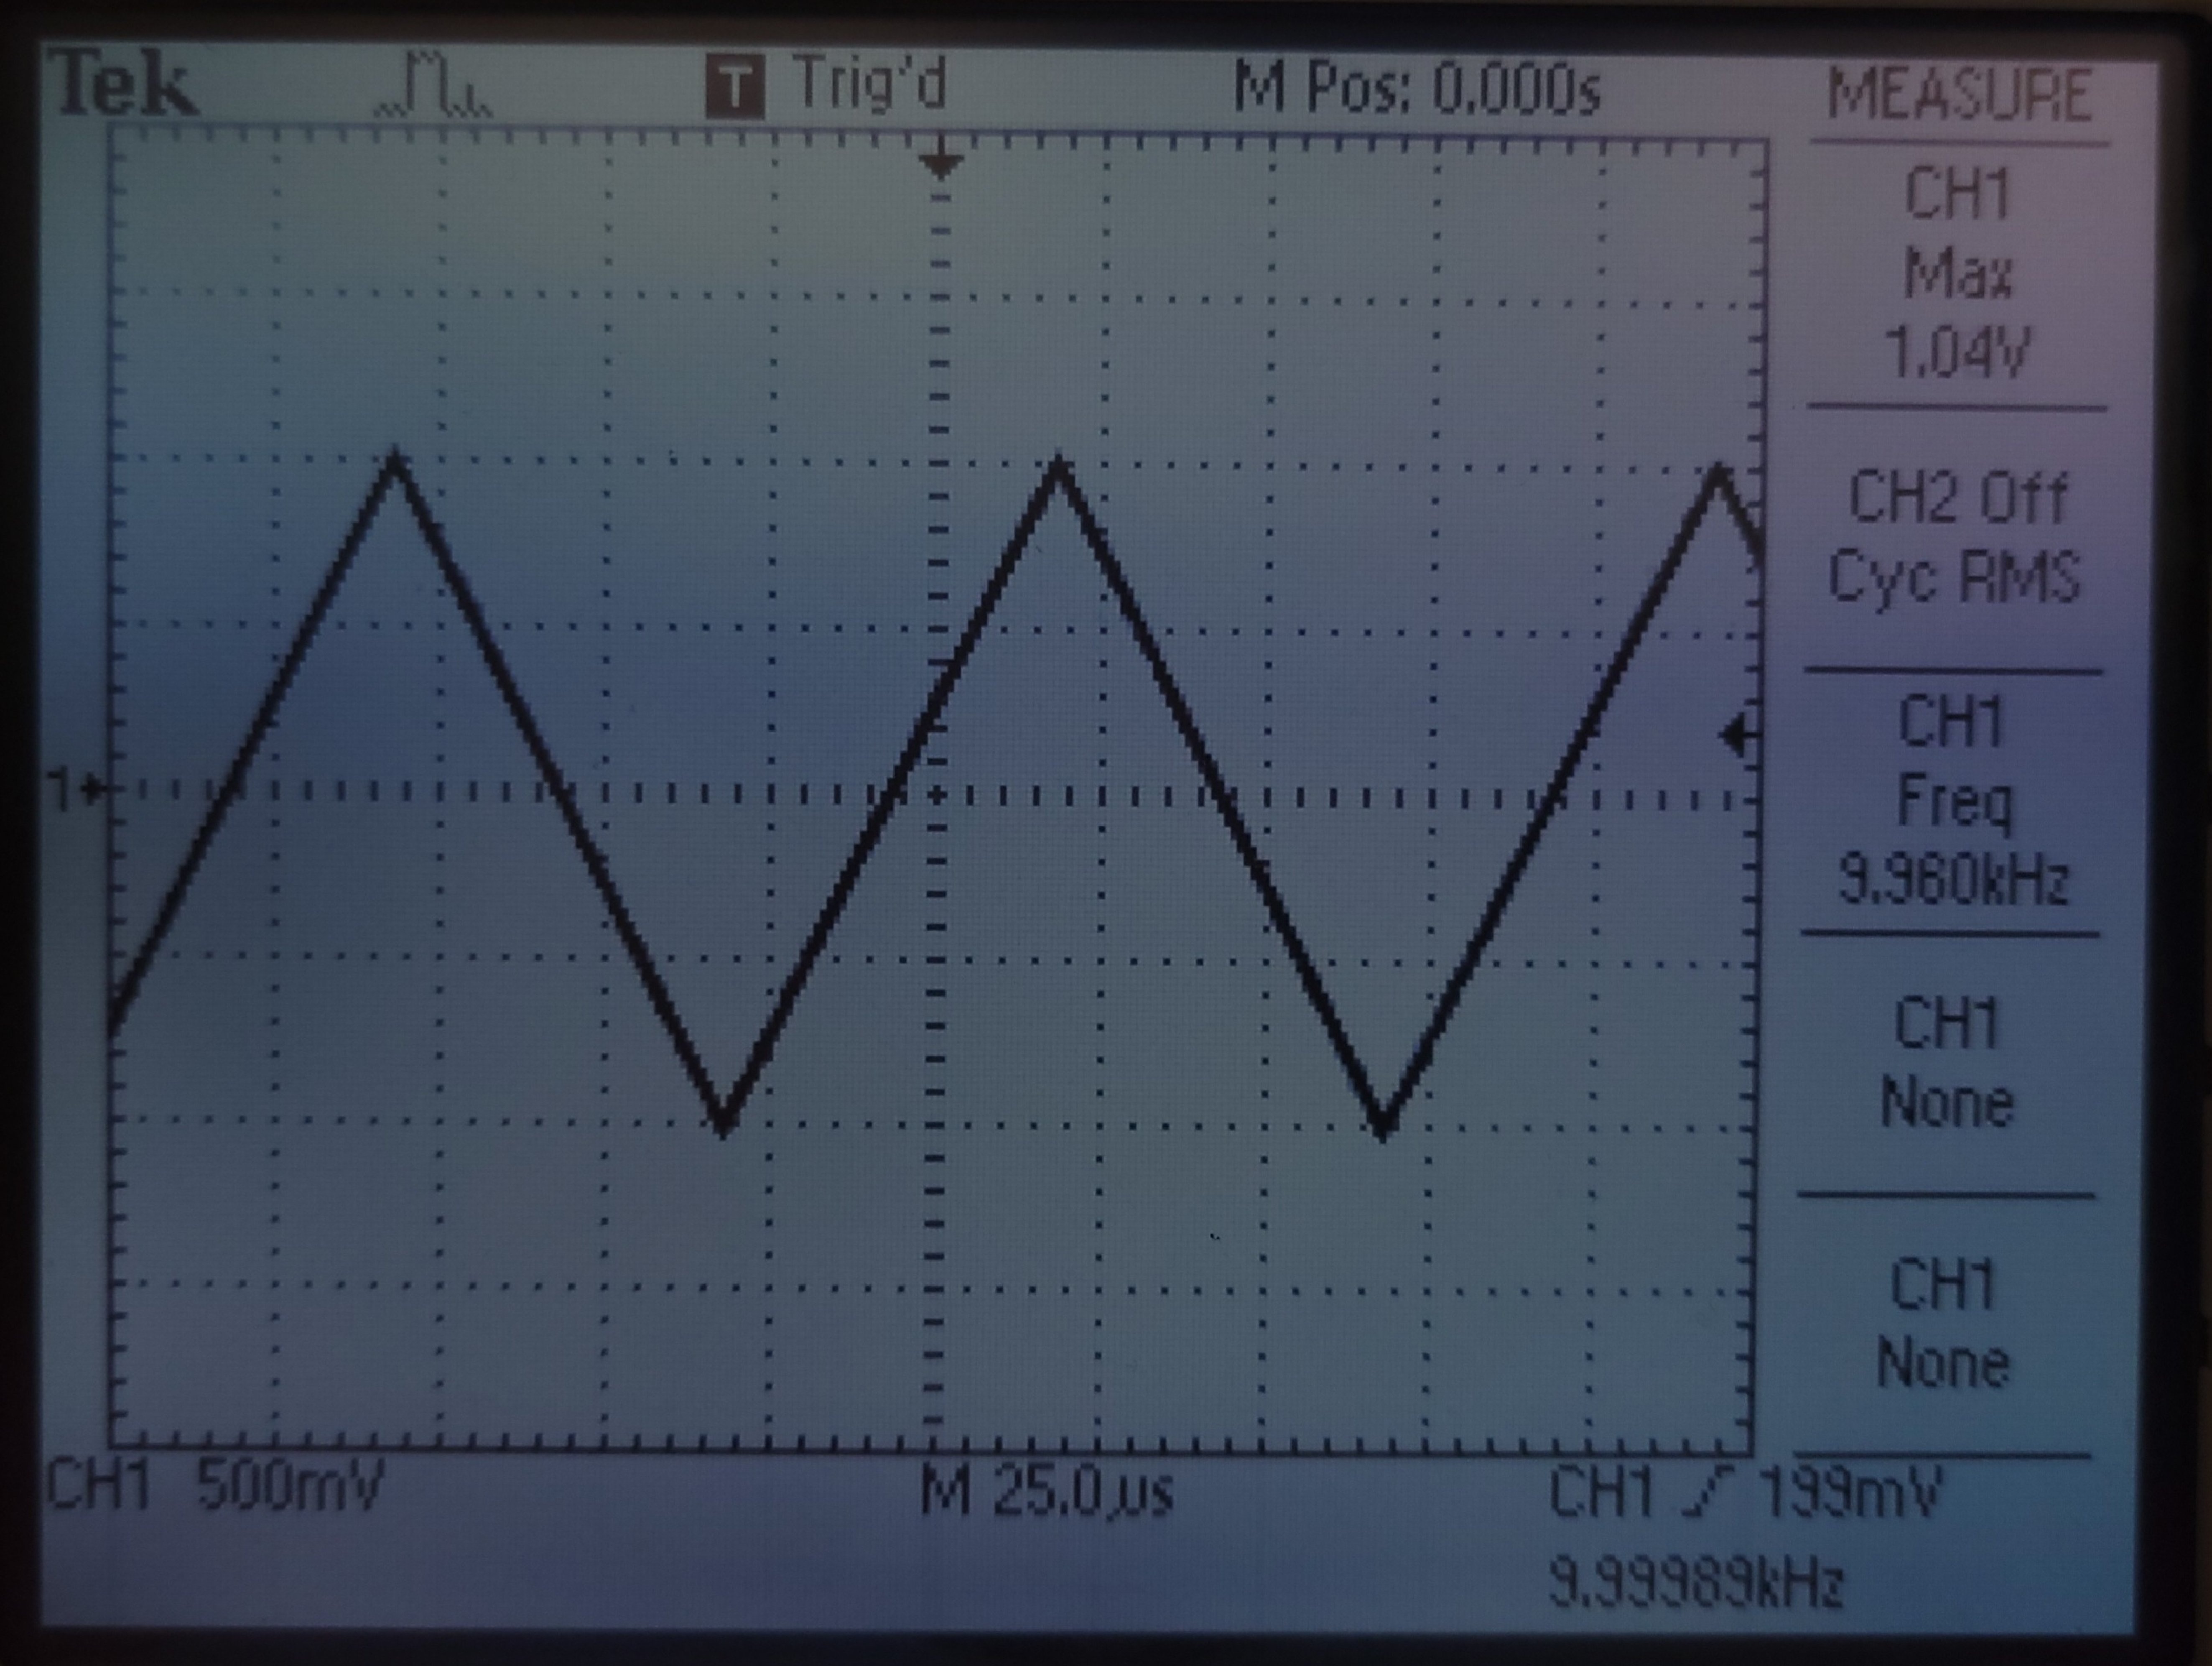
\includegraphics[width=\textwidth, page=1]{simple_waveform}
            \caption{TDS 1012 oscilloscope view}
            \label{fig:0.7}
        \end{minipage} \hfill
        \begin{minipage}{0.45\textwidth}
            \centering
            \includegraphics[width=0.8\textwidth, page=2]{simple_waveform}
            \caption{SR770 FFT Network Analyzer view}
            \label{fig:0.8}
        \end{minipage}\hfill
    \end{figure*}
    But the amplitude of the harmonics decreases by a factor of $1/n^2$. This power law makes the amplitude hard to read in the linear scale,
    but in the log scale, the amplitudes are clearly visible as shown in Fig. \ref{fig:0.9}.
    \begin{figure*}[ht]
        \centering
        \includegraphics[width=0.4\textwidth, page=3]{simple_waveform}
        \caption{SR770 LOG MAGNITUDE}
        \label{fig:0.9}
    \end{figure*}

\end{itemize}

\newpage

\paragraph*{Superposition of sine waves}

\begin{itemize}
    \item 770: 40 kHz, 1 V sine wave $\to$ SUMMER input A
    \item 33500B: 50 kHz, 2 V sine wave $\to$ SUMMER input B
    \item SUMMER output $\to$ 770 SIGNAL IN \& TDS 1012
\end{itemize}

\begin{figure*} [ht]
    \centering
    \includegraphics[width=0.5\textwidth]{fig1.png}
    \caption{Diagram of setup}
\end{figure*}

From the 770, we can easily see the two sine waves in the frequency domain as shown in Fig. [insert fig 0.11],
but the time domain (scope) does not clearly describe the summation of the two waves.

\paragraph*{Similar amplitude}
\begin{itemize}
    \item 770: 50 kHz, 1 V sine wave $\to$ SUMMER input A
    \item 33500B: 51 kHz, 1 V sine wave $\to$ SUMMER input B
\end{itemize}

In the full (100 kHz) span view, we can't see the two peaks.
To increase the frequency resolution, we can reduce the span in the 770 FREQ menu, 
but this will increase the acquisition time. 

e.g. a full span of 100 kHz has an acquisition time of 4 ms;
the `voltage sampling' rate is 256 kSa/s, or 256 samples per ms i.e. 1024 samples in 4 ms.

For our experiment, we set the span to 1.56 kHz to clearly see the two peaks, but this costs us
an acquisition time of 256 ms or $256 * \qty{256}{samples/ms} = 65536$ samples. This trade-off can be described by
the `frequency duration uncertainty principle':

\[\textrm{(frequency resolution achievable)} \cdot \textrm{(acquisition time required)} \geq  \textrm{a number}\]

The 770 magic number is
\begin{align*}
    \qty{100}{kHz} \cdot \qty{4}{ms} &\geq \qty{400}{kHz.ms}
\end{align*}
which we can use to find the minimum acquisition time for a given frequency resolution e.g. the 1.5625 kHz span required
\begin{align*}
    \textrm{(acquisition time req)} &\geq 400 / \textrm{(freq resolution)} \\
    &= 400 / 1.5625 = \qty{256}{ms}
\end{align*}

\paragraph*{Windowing \& Different amplitude}

Recommended windowing:
\begin{itemize}
    \item Uniform: close spanced peaks with similar amplitudes
    \item Flattop: accurate peak height measurement
    \item Hanning: good for spectral resolution
    \item BMH: good for weak peak near strong peak, but not the best resolution for top peak \& amplitude accuracy
\end{itemize}

\subsubsection*{Summary} 
\newpage
\chead{9/3/24}
\section{Signal Recovery Under Noise}

\subsection*{Chapter 6: Noise Waveforms}
\addcontentsline{toc}{subsection}{Chapter 6: Noise Waveforms}


\end{document}